\documentclass[11pt]{article}
\usepackage{graphicx}
\usepackage{hyperref}
\usepackage[dvipsnames, svgnames, x11names, hyperref]{xcolor}
\hypersetup{
	colorlinks,
	citecolor=Violet,
	linkcolor=Red,
	urlcolor=Blue}
\usepackage{natbib}
\usepackage{commath, amsmath}
\usepackage{siunitx}
\usepackage{gensymb}

\setlength{\textwidth}{6.5in}
\setlength{\headheight}{0in}
\setlength{\textheight}{8.0in}
\setlength{\hoffset}{0in}
\setlength{\voffset}{0in}
\setlength{\oddsidemargin}{0in}
\setlength{\evensidemargin}{0in}



\title{PS-7 sol}

\author{Nana Ama Nyamekye Darpaah}

\begin{document}
	
	\maketitle
	This is my GitHub link: \href{https://github.com/nnd2016/phys-ga2000.git}{Nana Ama's GitHub Link}
	
	\section{Question 1}
	
	The Lagrange Points are specific locations in space where the gravitational forces between two bodies of mass balance out hence objects sent to these locations stay put. The equation describing this point is expressed in Equation \ref{eq1} where $G$ is the gravitational constant, $m$ is the mass of the smaller object, $M$ is the mass of the bigger object, $\omega$ is the angular frequency of the orbit and $R$ is the distance between them.
	\begin{figure}[!h]
		
		\centering
		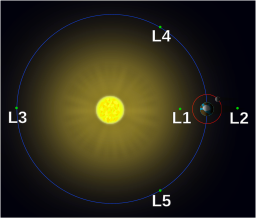
\includegraphics[width=0.53\linewidth]{lagrange_pic.png}
		\caption{Lagrange Points in the Sun-Earth System}\cite{website:wiki_lagrange}
		\label{fig:sun-earth}
		
	\end{figure}
	
	\begin{equation}
		\frac{GM}{(R-r)^{2}} + \frac{Gm}{(r)^{2}} = \omega^{2} r
		\label{eq1}
	\end{equation}
	The $\frac{GM}{r^{2}}$ term constitutes the force felt by the smaller mass $m$ due to the bigger mass $M$ and $\frac{GM}{(R-r)^{2}}$ is the force felt by the larger mass $M$ due to the smaller mass $m$.
	
	We know that 
	\begin{equation}
		m\omega^{2} R = \frac{GMm}{R^{2}}
	\end{equation}
	Hence
	\begin{equation}
		\omega^{2}  = \frac{GM}{R^{3}}
	\end{equation}

Inserting into Equation \ref{eq1}, we get
\begin{equation}
	\frac{M}{(R-r)^{2}} + \frac{m}{r^{2}} =  \frac{M(R-r)}{R^{3}}
	\label{eq4}
\end{equation}

The quintic equation is 
\begin{equation}
	\frac{M}{(R-r)^{2}} + \frac{m}{r^{2}} =  \frac{M(R-r)}{R^{3}}
	\label{eq4}
\end{equation}

Rescaling with $m' = m/M$ and $r' = r/R$, the new equation is
\begin{equation}
	\frac{m'}{(1-r)^{2}} + r - \frac{1}{r^{2}} =  0
	\label{eq5}
\end{equation}
The constants used were
\begin{itemize}
	\item Earth Mass = $5.974\times10^{24} $m
	\item Moon Mass = $7.384 \times 10^{22}$m
	\item Sun Mass = $1.988\times10^{30}$m
	\item Jupiter Mass = $1.898\times10^{27}$m
	\item Earth-Moon Distance = $3.844\times10^8$m
	\item Earth-Sun Distance = $1.496\times10^{11}$m
\end{itemize}

Equation \ref{eq5} was solved using the Newton's Method.
\begin{figure}[!h]
	
	\centering
	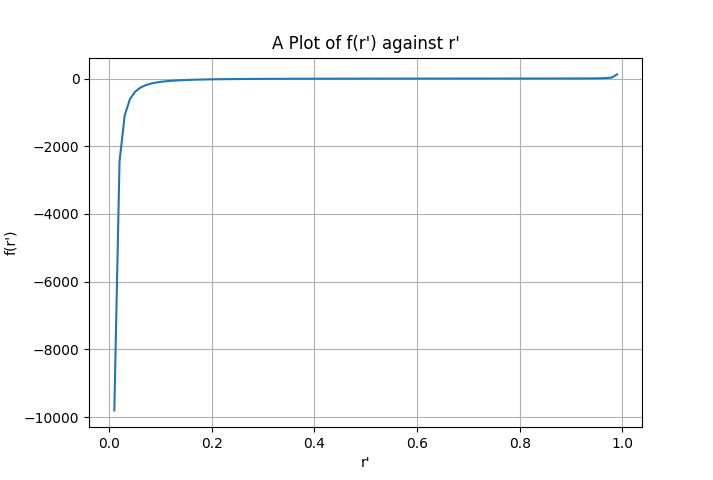
\includegraphics[width=0.83\linewidth]{lagrange.png}
	\caption{A Graph of the Earth-Moon System}
	\label{fig:earth-moon}
	
\end{figure}
From Figure \ref{fig:earth-moon}, it is seen that the minimum is very close to zero and hence the initial point was chosen to be $r' = 0.001$.


The Lagrange Points for the Earth-Moon, Sun-Earth and Jupiter-Sun systems were calculated to be $3.26231230 \times 10^{8}$m, $1.4812029 \times 10^{11}$m and $3.5876614 \times 10^{8}$m respectively, with the Jupiter mass planet orbiting the sun at the distance of the earth-sun system. The actual Lagrange points for the Earth-Moon and Sun-Earth system are $3.2639\times 10^8$m and $1.4811\times10^{11}$m respectively which can be seen to closely match the results calculated.

\section{Question 2}
 Brent's 1D minimization is a method which combines the golden ratio search and parabolic minimization method in order to find the minimum or maximum of a function. The analytical derivative of the function under consideration is was derived using the jax module. A graph of the function $y = (x-0.3)^{2}\exp(x)$ is plotted in Figure \ref{fig:brent}.
  
 \begin{figure}[!h]
 	
 	\centering
 	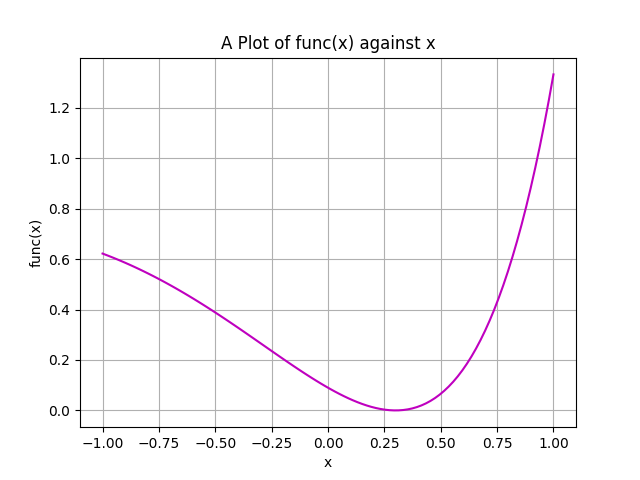
\includegraphics[width=0.83\linewidth]{brent.png}
 	\caption{A graph of func(x) against x}
 	\label{fig:brent}
 	
 \end{figure}
 
 From here, the initial bracketing points of $a=0, b=0.5, c=1$ were chosen.
 The Brent's 1D minimization method created yielded a minimum at $x = 0.299978016927797$ while that of scipy.optimize.brent had a minimum at $x = 0.3000000000124971$ which yields a difference of $2.1983084700083477\times 10^{-5}$.
 
 \cleardoublepage
 \renewcommand\bibname{References}
 \bibliographystyle{vancouver}
 \bibliography{ref}
 
\end{document}